
\subsection{Low Energy Channel}
\label{subsec:LowE}
This analysis channel relies on the re-analysis of run~II data described in~\cite{xe100_run_combination}. The ROI, the background 
expectation models, data selections and their acceptances are mostly unchanged and so are only briefly summarized here. Differences with respect to said results are highlighted when present.

The region of interest for this channel spans the ROI in the ($y,cS1$)-plane and is shown in Figure~\ref{fig:phasespace}.  The lower 
bound on $y$ corresponds to a 3\,$\sigma$ acceptance quantile (as a function of cS1) of a 20~GeV WIMP mass signal model assuming an $\mathcal{O}_1$ (SI) interaction, while the upper bound is fixed at y\,=\,2.7.
The range in cS1 is selected as 3 to 30\,PE. This ROI is further divided into sub-regions on each WIMP mass and operator (also called bands). These bands are arranged to achieve constant expected signal density in each region, as described in~\cite{xe100_run_combination}.

\begin{figure}[]
\begin{minipage}{1\linewidth}
\centerline{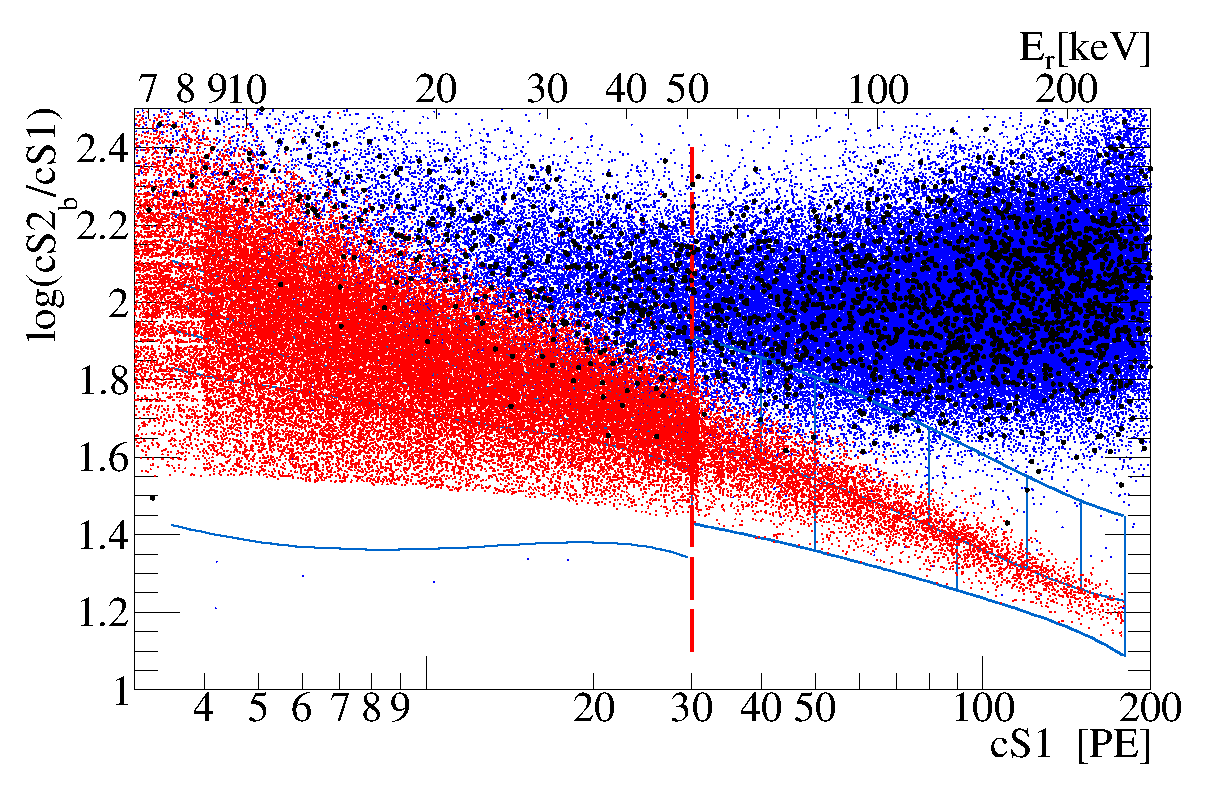
\includegraphics[width=1\linewidth]{Figures/eft_sr.eps}}
\end{minipage}
\caption{Summary of regions of interest, backgrounds, and observed data. ER calibration data, namely $^{60}\mathrm{Co}$ and $^{232}\mathrm{Th}$ data is shown as blue dots. NR calibration data ($^{241}$AmBe) is shown as red dots. Dark matter search data is shown as black dots. The red dashed line is the threshold between the low and high energy channels. The lines in blue are the bands. For the low-energy channel these are operator and mass dependent, but are shown here for a 50~GeV/$c^2$ WIMP using the $\mathcal{O}_1$ operator. For the high-energy region, the 9 analysis bins are presented also in blue lines; the top left bin in this region is bin 1, the top right is bin 6, the bottom left is bin 7 and bottom right is bin 9. 
In Sec.~\ref{sec:Results} we show similar data but for regions above the upper range of this analysis, going up to 1000\,PE in cS1, for completeness as part of final unblinding of XENON100 data. 
}
\label{fig:phasespace}
\end{figure}  


Other than falling into the ROI, an event should fulfill several additional selection criteria (cuts). Data quality and selection cuts are defined to remove events with poor data quality or noisy signals, a time-coincident signal in the outer LXe veto, S2 signals below threshold, multiple-scatters, and positions outside a predefined fiducial volume of 34 kg. In addition, this analysis channel uses the post-unblinding cuts and data reprocessing described in~\cite{xe100_run_combination}. More details on these selection criteria and their relative WIMP signals acceptances can be found in~\cite{Aprile:2012vw,xe100_run_combination}. 


%%%%% MAYBE THIS CAN BE COMMENTED OUT %%%%%%
To summarize the main new features in this analysis, data is reprocessed with an improved (S1,S2) classification algorithm, and a new cut targeted to suppress data periods with non-random occurrence of lone-S1 (an S1 without 
any correlated S2) events is applied. 
%%%%%%%%%%%%%%%%%%%%%%%%%%%%%%%%%%%%%%%%%%%%%
Finally, this channel does not employ a variable lower S1 threshold as a function of the event position in the TPC, but a fixed 
lower threshold cut on cS1 at 3\,PE, converse to what was done in~\cite{xe100_run_combination}.

The expected background is modeled separately for ER and NR contributions which are then scaled to exposure and added together.
The NR background is estimated by Monte Carlo simulation and accounts for the radiogenic and cosmogenic neutron
contributions~\cite{Aprile:2013tov}.
%neutrons from ambient materials and neutrons induced by cosmic ray showers. 
The ER background is parametrized as the linear combination of Gaussian-shaped and non-Gaussian components.
The first is obtained via a parametric fit of the $^{60}$Co and $^{232}$Th calibration data, as discussed in~\cite{xe100_run10_si}.
In contrast, the expected distribution and yields for the non-Gaussian population, consisting of anomalous events such as those 
presenting incomplete charge collection or accidental coincidence of uncorrelated S1s and S2s,  
are evaluated via dedicated techniques described in~\cite{xe100_run_combination}.

Systematic uncertainties on the background model arising from the Gaussian parametrized fit plus the normalisations of the NR and non-Gaussian components have been evaluated and propagated to each band. These errors are small with respect to the statistical uncertainties of each band, which are taken as the overall uncertainty ~\cite{xe100_run_combination} as discussed in Sec.~\ref{sec:LikelihoodFunction}.

